
% !TEX root = ../paper.tex

\section{Introduction}

This chapter is based on material from the following publication:

\begin{mdframed}
\begin{center} 
    \bibentry{van2024distributional} 
\end{center}
\end{mdframed}

\begin{figure}[!ht]
	\begin{center}
	\centerline{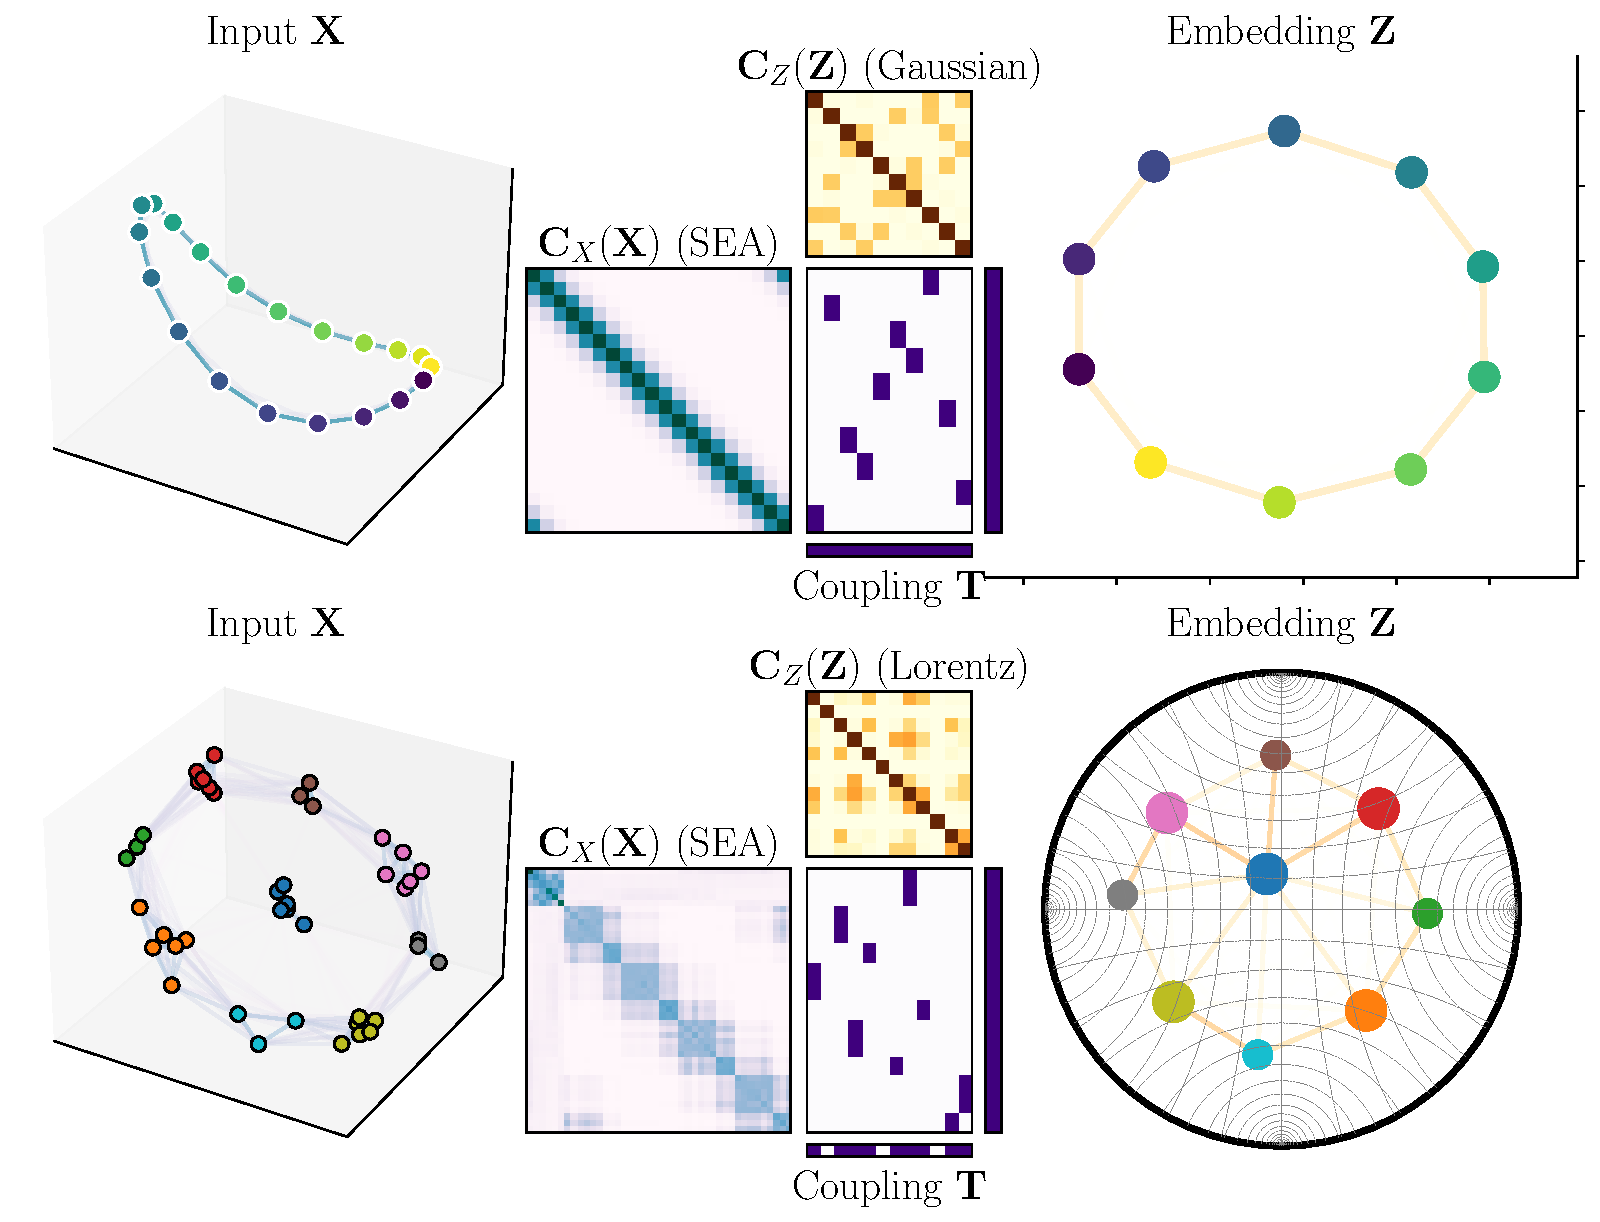
\includegraphics[width=\columnwidth]{figures/DistR/fig_general.pdf}}
	\caption{\textbf{Illustration of our \ref{eq:Dist-DR} method} on two toys examples: points arranged on a circle ({\em top row}) and clusters with varying sizes ({\em bottom}) both in 3 dimensions. {\em Middle column}: input similarity matrix $\mC_X(\mX)$ and final resulting embedding similarity $\mC_Z(\mZ)$. Both are coupled through the coupling matrix $\mT$ (depicted in purple, with its marginals)}
	\label{fig:general_idea}
	\end{center}
	\vskip -0.3in
\end{figure}

This work addresses \Cref{prob:ot_unsupervised} and aims to provide a general formulation of unsupervised representation learning methods as an OT variational problem over a measure. Of particular interest are clustering and dimensionality reduction approaches, both of which are popular ways to summarize datasets. Interestingly, methods from both families share many similitudes, %among which is
including the construction of a similarity graph between input samples. In clustering, many popular approaches design a reduced or coarsened version of the initial similarity graph while preserving some of its spectral properties~\citep{von2007tutorial, schaeffer2007graph}. 
%attributes related to the graph spectrum 
In DR, the goal is to solve the inverse problem of finding low-dimensional embeddings that generate a similarity graph close to the %initial
one computed from input data points \citep{ham2004kernel,hinton2002stochastic}.
%With so many similarities
Our work builds on these converging viewpoints and addresses the following question: \emph{can DR and clustering  be expressed in a common and unified framework ?}

\paragraph{A distributional perspective.} To answer this question, we
propose to look at both problems from a distributional point of view, treating the data as an empirical probability distribution
$\mu=\frac{1}{N}\sum_i\delta_{\vx_i}$. 
% instead of a data matrix. 
This enables us to consider statistical measures of similarity such as Optimal Transport (OT), which is at the core of our work.
On the one hand, OT and clustering are strongly related.
The celebrated K-means approach can be seen as a particular case of minimal Wasserstein estimator where a distribution of $n$ Diracs is optimized \textit{w.r.t} their weights and positions \citep{Canas12}. Other connections between spectral clustering and the OT-based Gromov-Wasserstein (GW) distance have been recently developed in \citep{chowdhury2021generalized,chen2023gromov,vincent2021semi}. On the other hand, the link between DR and OT has not been explored yet. DR methods, when modeling data as distributions,
usually focus on joint distribution between samples within each space separately, see \eg \Cref{chapter:SNEkhorn} of this thesis or \citep{lu2019doubly}.
Consequently, they do not consider couplings to transport samples across spaces of varying dimensions. %To the best of our knowledge, DR methods, when modeling data as distributions,
%focus on joint distribution between samples within each space separately, see \eg \citet{van2023snekhorn} or \citet{lu2019doubly}.
%However, they do not consider couplings to transport samples across spaces of varying dimensions,% thus the link between DR and OT has not been explored yet.
% they do not consider a
% minimal divergence estimator and 

\paragraph{Outline.} In this chapter, we propose to bridge this gap by
proposing a novel and general distributional framework that encompasses both DR and clustering
as special cases. We notably cast those problems as finding a reduced distribution that minimizes the GW divergence from the original empirical data distribution.
Our method proceeds by first constructing an input similarity matrix
$\mC_X(\mX)$ that is matched with the embedding similarity $\mC_Z(\mZ)$ through
an OT coupling matrix $\mT$. The latter establishes correspondences between
input and embedding samples. We illustrate this principle in
Figure~\ref{fig:general_idea} where one can notice that $\mC_Z(\mZ)$ preserves
the topology of $\mC_X(\mX)$ with a reduced number of nodes. The adaptivity of
our model that can select an effective number of cluster $<n$, is visible in the
bottom plot, where only the exact number of clusters in the original data ($9$ out of the $12$
initially proposed) is automatically recovered. Our method can operate in any embedding space, which is illustrated by
projecting in either a 2D Euclidean plane or a Poincaré ball as embedding
spaces.

We show that this framework is versatile and allows to recover many popular DR
methods such as the kernel PCA and neighbor embedding algorithms, but also clustering 
algorithms such as K-means and spectral clustering. We first prove in Section
\ref{sec:DR_as_OT} that DR can be formulated as a GW projection problem under
some conditions on the loss and similarity functions. We then propose in Section
\ref{sec:DDR} a novel formulation of data summarization as a minimal GW estimator that allows
to select both the dimensionality of the embedding $d$ (DR) but also the number of Diracs
$n$ (Clustering).
% hence providing jointly DR and clustering. 
%Finally, we show in Section \ref{sec:exps} the practical interest and generality of our approach by evaluating its performance on a joint DR/Clustering task and comparing it to existing methods.
Finally, we show in section \ref{sec:exps_distr} the practical interest of our approach, which regularly outperforms its competitors for various joint DR/Clustering tasks.
% \hva{à atténuer un peu:}
% We also illustrate the generality by investigating particularly novel DR methods that optimize the GW divergence in an Eulerian way, with a reduced distribution of fixed support \nc{such as} regular grids (images) or on other supports that can encode prior knowledge.

% Summarizing a dataset in an unsupervised way is of utmost importance in modern machine learning pipelines \citep{donoho2000high}. Reduced data representations offer numerous advantages, including improved pattern and structure recognition as well as faster processing for downstream tasks \citep{pochet2004systematic, mendible2020dimensionality, cantini2021benchmarking}.

% To construct such representations, one can either reduce the sample size by aggregating points together (referred to as \emph{clustering}) or reduce the feature dimensionality \textit{i.e.}\ performing \emph{dimensionality reduction} (DR). 
% Both tasks are actively studied topics and %interestingly
% their inner workings share key mechanisms, %among which is
% like the construction of a similarity graph between input samples.
%  \cvc{(missing high level motivation about why one would want to do so?)}
% However current formulations of DR do not permit adapting the sample size of the resulting embedding. 
% In other words, there does not exist a consistent model allowing to adapt current state-of-the-art DR algorithms to simultaneously perform clustering. As a result, clustering and DR are performed sequentially \cvc{(need to outline limitations of sequential approach)}. 
% In cell biology, for instance, similar cells are grouped into \emph{metacells} \citep{baran2019metacell} that are then embedded onto a low-dimensional space for visualization and other downstream tasks.
% This may result in clusters that are not adapted to the final embedding space and vice versa \citep{liu2022joint} \cvc{(maybe the example should come sooner)}.

% \textbf{Contributions.}
% In this work, we uncover the link between popular DR methods and the Gromov-Wasserstein optimal transport problem \citep{memoli2011gromov}. \cvc{This leads us to frame DR as a novel optimization problem over any discrete distributions, \emph{a.k.a} Distributional Dimensionality Reduction, that provides a first grounded approch for joint DR and clustering.} This novel characterization allows us to frame DR as an optimization problem over discrete distributions offering enhanced flexibility. In particular, it allows one to choose the resolution of the output thus providing a grounded approach for joint dimensionality reduction and clustering. Our contributions can be summarized as follows.
% \begin{itemize}
% 	\item In \Cref{sec:DRasOT}, we provide conditions on the loss and similarity functions under which DR can be equivalently formulated as the GW projection of the empirical data distribution.
% 	\item In \Cref{sec:DDR}
	
% 	\item In \Cref{sec:exps}, we showcase the relevance of our approach for summarizing real datasets composed of images and single-cell data. Compared with existing benchmarks, we show that our model achieves the best trade-off between structure preservation and homogeneity of the obtained clusters.
% \end{itemize} 